% !TeX spellcheck = en_GB
% Template for ICASSP-2010 paper; to be used with:
%          mlspconf.sty  - ICASSP/ICIP LaTeX style file adapted for MLSP, and
%          IEEEbib.bst - IEEE bibliography style file.
% --------------------------------------------------------------------------
\documentclass{article}
\usepackage{amsmath,graphicx,02460}
\usepackage{amssymb}
\usepackage{algorithm}
\usepackage{algpseudocode}
\usepackage{bm}

\usepackage[dvipsnames]{xcolor}

\usepackage{pgf,tikz}
\usepackage{localpie}
\usetikzlibrary{arrows}
\usetikzlibrary{decorations.markings}

\usepackage{url}
\allowdisplaybreaks
\PassOptionsToPackage{hyphens}{url}\usepackage{hyperref}
\def\UrlBreaks{\do\/\do-}

\toappear{02460 Advanced Machine Learning, DTU Compute, Spring 2022}


\newcommand{\code}[1]{{\texttt{\small#1}}}
\newcommand{\numberthis}{\addtocounter{equation}{1}\tag{\theequation}}
\newcommand{\acomm}[1]{\hspace{2.5cm}\text{#1}}
\newcommand{\low}[1]{\ensuremath{_\textup{#1}}}

\newcommand{\andim}{\textup{ and }}
\newcommand{\raq}{\Rightarrow\quad}
\newcommand{\lraq}{\Leftrightarrow\quad}
\newcommand{\qandq}{\quad\wedge\quad}
\newcommand{\qorq}{\quad\vee\quad}
\newcommand{\diff}[2]{\ensuremath{\frac{\md #1}{\md #2}}}
\newcommand{\md}{\ensuremath{\text{d}}}

\newcommand{\ctp}[1]{\ensuremath{\cdot10^{#1}}}
\newcommand{\reci}{\ensuremath{^{-1}}}
\newcommand{\twopow}{\ensuremath{^{2}}}
\newcommand{\re}[1]{\ensuremath{^{#1}}}

\newcommand{\me}{\ensuremath{\operatorname{e}}}
\newcommand{\eul}[1]{\ensuremath{\me^{#1}}}
\newcommand{\len}[1]{\ensuremath{\left\lvert#1\right\rvert}}
\newcommand{\half}{\ensuremath{\frac{1}{2}}}
\newcommand{\third}{\ensuremath{\frac{1}{3}}}
\newcommand{\fourth}{\ensuremath{\frac{1}{4}}}
\newcommand{\transpose}[1]{\ensuremath{#1^{\textup T}}}

\newcommand{\NN}{\ensuremath{\mathbb N}}
\newcommand{\ZZ}{\ensuremath{\mathbb Z}}
\newcommand{\QQ}{\ensuremath{\mathbb Q}}
\newcommand{\RR}{\ensuremath{\mathbb R}}
\newcommand{\CC}{\ensuremath{\mathbb C}}
\newcommand{\LL}{\ensuremath{\mathbb L}}
\newcommand{\PP}{\ensuremath{\mathbb P}}

\newcommand{\unit}[1]{\ensuremath{\:\text{#1}}}
\newcommand{\pro}{\ensuremath{\unit{\%{}}}}

%Kommandoer til ændring af ligestillingsmargner
\newcommand{\jl}[1]{\multicolumn{1}{l}{#1}}
\newcommand{\jc}[1]{\multicolumn{1}{c}{#1}}
\newcommand{\jr}[1]{\multicolumn{1}{r}{#1}}
\newcommand{\jls}[1]{\multicolumn{1}{l|}{#1}}
\newcommand{\jcs}[1]{\multicolumn{1}{c|}{#1}}
\newcommand{\jrs}[1]{\multicolumn{1}{r|}{#1}}

\title{20 Raspberry Pi's, One Model: Federated Learning On Real Hardware}
\name{Søren Winkel Holm, Asger Laurits Schultz, Gustav Lang Moesmand}
\address{Technical University of Denmark}
%
%
\begin{document}
%\ninept
%

\maketitle
%

\begin{abstract}
    Federated Learning (FL) is emerging as an essential mechanism for assuring user privacy in large-scale machine learning (ML) \cite{kai2021advances}.
    Important use-cases of this learning paradigm run on a federation of real-world user devices, but in the literature, FL is often simulated in an artificial computing cluster environment \cite{kai2021advances,mcmahan2017communication,lin2020ensemble}.
    Seeking to capture the unique FL problems and trade-offs when running on physical hardware, we set up 20 Raspberry Pi's acting as user devices.
    Using this experimental setup, we perform an empirical study of the influence of key hyperparameters of the FedAvg \cite{mcmahan2017communication} algorithm.
    In the case of the number of local epochs on clients, the physical timings allow us to identify a trade-off between time spent on communication and local computation.
    Testing robustness against imbalanced data across the clients and noisy data, we highlight the potential of using stronger aggregation schemes than weight averaging by implementing the FedDF \cite{lin2020ensemble} algorithm.
\end{abstract}

\section{INTRODUCTION}
\label{sec:intro}
Large-scale surveys have shown that the growing use of Artificial Intelligence (AI) has resulted in a widespread fear of loss of personal privacy \cite{beuc2020consumers, west2018survey}.
As part of a general push towards safer AI, large tech companies such as Google and Apple have employed FL methods in cases including Siri, Google Chrome, and Gboard \cite{kai2021advances}.

The term FL covers distributed ML setups where multiple clients collaborate in learning from local datasets which are not exchanged and where a central server aggregates local updates \cite{kai2021advances, mcmahan2017communication}.
Aggregation by iteratively averaging weights from models, each produced by training for several local epochs on each client, is known as the formative \emph{FedAvg} \cite{mcmahan2017communication} algorithm.
For faster and more stable convergence, additional aggregation methods have been developed, including the ensemble distillation algorithm \emph{FedDF} \cite{lin2020ensemble}. 
We refer to Kairouz et al. for an overview of the field \cite{kai2021advances}.

Across this rich literature, many benchmarks of FL performance over algorithmic choices exist but are often performed by simulating the federation on central compute clusters \cite{lin2020ensemble}.
In this project, we seek to capture the unique hardware setup of FL use-cases such as smartphones, where a number of computationally weak edge devices hold the data.
This is achieved by performing local training of a convolutional neural network (CNN) on 20 Raspberry Pi devices over which CIFAR-10 \cite{alex2009learning} is divided and aggregating these locally trained models centrally using FedAvg.
The project aims to investigate the impact of FedAvg hyperparameters, including the number of clients per communication round and local epochs on convergence time, analyse aggregation robustness against imbalanced and noisy data, and uncover performance trade-offs in the physical hardware setting.

\section{METHODS}%
\label{sec:methods}

\subsection{FL Methods}
We implemented FL by setting up $K$ clients each with a disjoint training dataset partition of size $n_k$.
A global model, $\mathcal M_G$, was initialised and maintained on the central server, and for $L$ rounds, dubbed \emph{communication rounds}, $S \leq K$ clients were sampled, each receiving a copy of $\mathcal M_G$.
Each client performed $E$ local epochs of learning before returning the updated local model $\mathcal M_k$ to the server.

In FedAvg, the server aggregated the $S$ returned models by averaging over all model weights, yielding a new global model to be sent out for the next communication round, minimizing an implicit objective function $f$ of model weights $\mathbf w$ when using loss function $\ell$:
\begin{equation*}
    f(\mathbf w) = \sum_{k=1}^K \frac{n_k}{n_{\text{total}}} F_k(\mathbf w),\ \ 
    F_k(\mathbf w) = \frac 1 {n_k} \sum_{i=1}^{n_k} \ell (x_i, y_i; \mathbf w),
\end{equation*}
in which $F_k(\mathbf w)$ is the objective of the $k$'th client \cite{mcmahan2017communication}.

For an alternative aggregation method, we implemented the FedDF algorithm, where the FedAvg's weight averaging is replaced by running ensemble distillation for model fusion using an unlabeled dataset similar to the training datasets \cite{lin2020ensemble}.
Copying the hyperparameters from \cite{lin2020ensemble}, $\mathcal M_G^{(l + 1)}$ was produced by distilling the $S$ local models $\mathcal M_{k_i}^{(l)}$ for $10^4$ batch updates against a Kulback-Leibler (KL) divergence criterion with a batch size of $128$ and a learning rate of $10^{-3}$ used for Adam optimization with cosine annealing \cite{losh2016sgdr,kingma2015adam}.
Early stopping was implemented by calculating KL loss against an unlabeled validation set every $10^3$ updates and terminating if evaluation loss did not fall.
The CIFAR-100 dataset was used for distillation \cite{alex2009learning}.

\subsection{Physical Devices}
The project setup, shown in Figure \ref{fig:setup}, was divided into two parts A central high-performance cluster (HPC) and 20 Raspberry Pi 3B's, each with 1 GB memory and a quad-core 1.2 GHz CPU.
Crucially, the Pi's were located on a network separate from the HPC to simulate a more realistic communication overhead.
The HPC server was responsible for aggregating the local models trained by the Pi's and evaluating the resulting global model $\mathcal M_G$.
The code was designed not to require physical devices, so experiments without hardware timing were run on an NVIDIA A100 for faster training time and a reduced power bill.

Every Pi ran a Flask server that transferred models, ran local training and broadcast running memory usage; an important consideration when running on such resource-limited devices.
The Flask server also had a route for sending commands to allow primitive over-the-air-update functionality.

The Raspberry Pi setup was able to run experiments where $K > 20$, that is, maintaining more than 20 clients and thus dataset partitions with the constraint of no more than 20 clients being sampled each round: $S \leq 20$.
This was done by storing all $K$ client datasets on every device, and in each communication round $l$, assigning each of the $S$ sampled client datasets to a Raspberry Pi.

The Pi's were connected to a switch which was connected via cable to the router.
When turning off the switch, the Pi's were set to connect via Wi-Fi instead, allowing tests of the impact of communication overhead in two cases: under relatively fast Ethernet and relatively slow Wi-Fi.
For reference, the network used had a bandwidth of 100/100 Mbit/s, all of which was utilised on Ethernet, but only about 40\pro\ on Wi-Fi.

\begin{figure}[htb!]
    \centering
    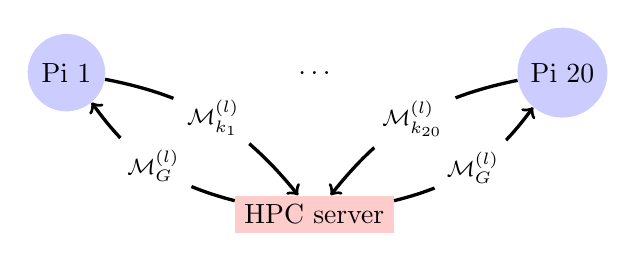
\begin{tikzpicture}[scale=.9,auto=center,every node/.style={circle}]

\tikzstyle{client}=[fill=blue!20];
\tikzstyle{server}=[fill=red!20,style=rectangle];
\tikzstyle{t}=[fill=red!0];

\node[server] (s) at (0,0) {HPC server};  
\node[client] (c1) at (-3.5,2)  {Pi $1$}; 
\node[t] (te) at (0, 2) {$\ldots$};
\node[client] (c2) at (3.5,2)  {Pi $20$};  

\path[->] (s) edge[very thick, bend left=20] node[midway, fill=white] {\footnotesize $\mathcal M_G^{(l)}$} (c1);
\path[->] (s) edge[very thick, bend right=20] node[midway, fill=white] {\footnotesize $\mathcal M_G^{(l)}$} (c2);

\path[->] (c1) edge[very thick, bend left=20] node[midway, fill=white] {\footnotesize $\mathcal M_{k_1}^{(l)}$} (s); 
\path[->] (c2) edge[very thick, bend right=20] node[midway, fill=white] {\footnotesize $\mathcal M_{k_{20}}^{(l)}$} (s); 


\end{tikzpicture}

    \caption{
        Our federated setup performing updates at communication round $l$, at which $S\leq 20$ clients are sampled, each corresponding to a dataset partition $k_1\ldots k_{S}$.
        Raspberry Pi 1 trains a model as client $k_i$, and Raspberry Pi 20 as $k_j$.
    }
    \label{fig:setup}
\end{figure}\noindent

\subsection{Deep Learning Problem}
As an example learning problem, we chose the CIFAR-10 computer vision (CV) task of classifying $32\times 32$ images into object classes such as birds, cats, and aeroplanes \cite{alex2009learning}.
Due to device memory limits, all images were greyscaled.
The training dataset contains 5K images for each of the 10 label.

For the model $\mathcal M$, we chose a network with two convolutional layers followed by two linear layers, which is further detailed in Appendix \ref{app:model}.
The model was limited in size to accommodate the strict memory limits on the Raspberry Pi's.

Optimization for the $E$ local epochs on each device was performed by using the Adam optimizer \cite{kingma2015adam} with a learning rate $\eta$, which was decayed every local epoch: $\eta\leftarrow\gamma\eta, \gamma\le 1$.

\subsection{Data Imbalance and Noise}
\subsubsection{Dirichlet sampling}
The total training dataset was divided into $K$ evenly sized partitions among all the clients.
In practice, dataset class balance can rarely be assumed in the FL setting \cite{kai2021advances}.
In order to simulate varying levels of imbalance, the Dirichlet distribution, $\operatorname{Dir}(\bm\alpha)$, was used.
The length of the parameter vector  $\bm\alpha$ corresponds to the number of labels, 10, and we let $\alpha_i=\alpha$.
Every sample $\bm\pi\sim\operatorname{Dir}(\bm\alpha)$ is a probability distribution over labels and $\alpha$ determines the uniformity of this distribution.
For $\alpha\to0$, one label dominates, where as for $\alpha\to\infty$, $\bm\pi$ will be increasingly uniform, as exemplified in Appendix \ref{app:dirplots}.
For $\alpha=1$, every possible $\bm\pi$ is equally likely.

$\bm\pi$ was sampled for every client, making the label distribution Dirichlet for every client.
To keep the client datasets disjoint while using a maximal part of the total dataset, we created a client-balancing Dirichlet sampling algorithm described in detail in Appendix \ref{app:diralg}.

As a comparative baseline, we also simulate random partitions, denoted iid. following literature \cite{lin2020ensemble}.

\subsubsection{Noisy data}
To simulate the fact that some user devices can be unreliable, we tested the concept of noisy clients.
The training data on a noisy client had all labels replaced with randomly chosen classes, removing all signal.
We tested performance over the number of noisy clients $N_K\leq K$ to simulate erroneous or even adversarial clients.

\subsection{Evaluation}
We performed experiments using FedAvg testing the effects of four variables: The number of clients sampled ($S$), the class balance ($\alpha$), the number of local epochs ($E$) and the number of noisy clients ($N_K$). 
Furthermore, the experiments regarding class balance and noisy clients were also run using the FedDF algorithm.

The experiments varying local epochs were repeated on the physical federation of Raspberry Pi's, both on Ethernet and Wi-Fi.
This was chosen because altering this parameter changes the runtime of each communication round, while the behaviour for other tested parameters was approximately the same whether using the number of communication rounds or wall time as the $x$-axis.

All experiments used the baseline listed in Table \ref{tab:baseline} except for the parameter being varied in each experiment.
These were chosen based on existing literature, in particular, \cite{mcmahan2017communication,lin2020ensemble}, and limited pilot experimentation.

\begin{table}[htb!]
    \centering
    \begin{tabular}{ccccccccc}
        $K$ & $S$ & $\alpha$ & $E$ & $L$ & $N_K$ & $B$ & $\eta$ & $\gamma$\\
        \hline
        40 & 20 & 1 & 20 & 20 & 0 & 16 & $5\ctp{-4}$ & $0.995$
    \end{tabular}
    \caption{Baseline parameters used for all experiments.
        Here, $B$ refers to the training batch size.}
    \label{tab:baseline}
\end{table}

\section{RESULTS}%
\label{sec:results}
Figure \ref{fig:rpi-local-epochs} shows the experiments run on the Pi setup.
Note that these experiments are limited by time and have thus run different numbers of communication rounds.
\begin{figure}[htb!]
    \centering
    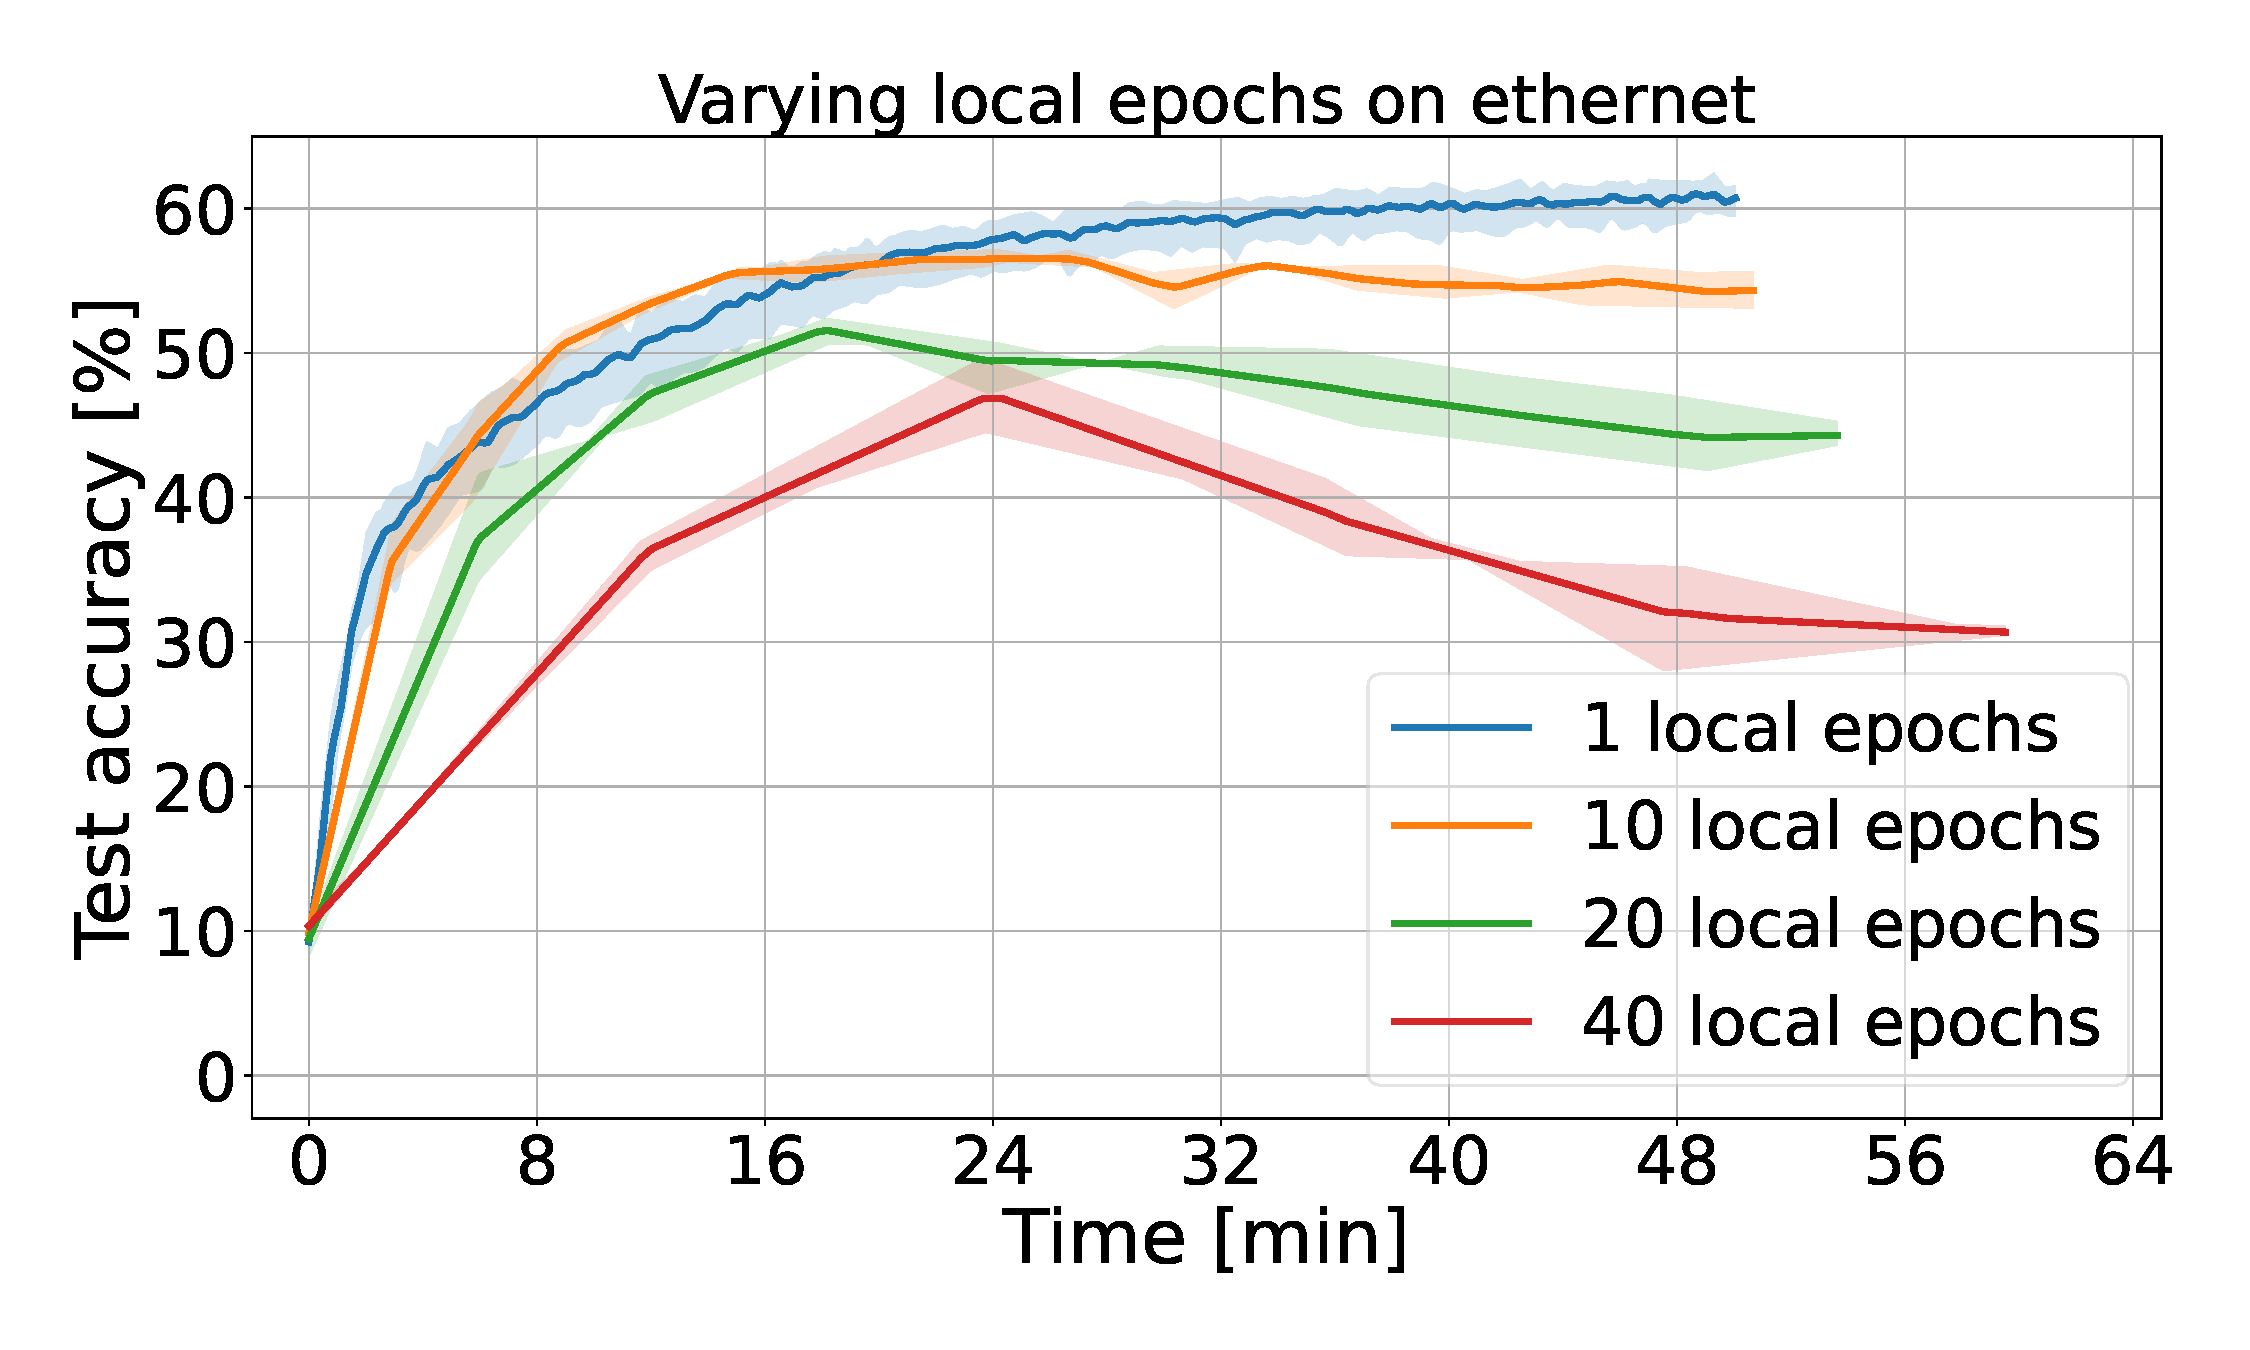
\includegraphics[width=\linewidth]{imgs/time_avg_local_epochs_ethernet.pdf}
    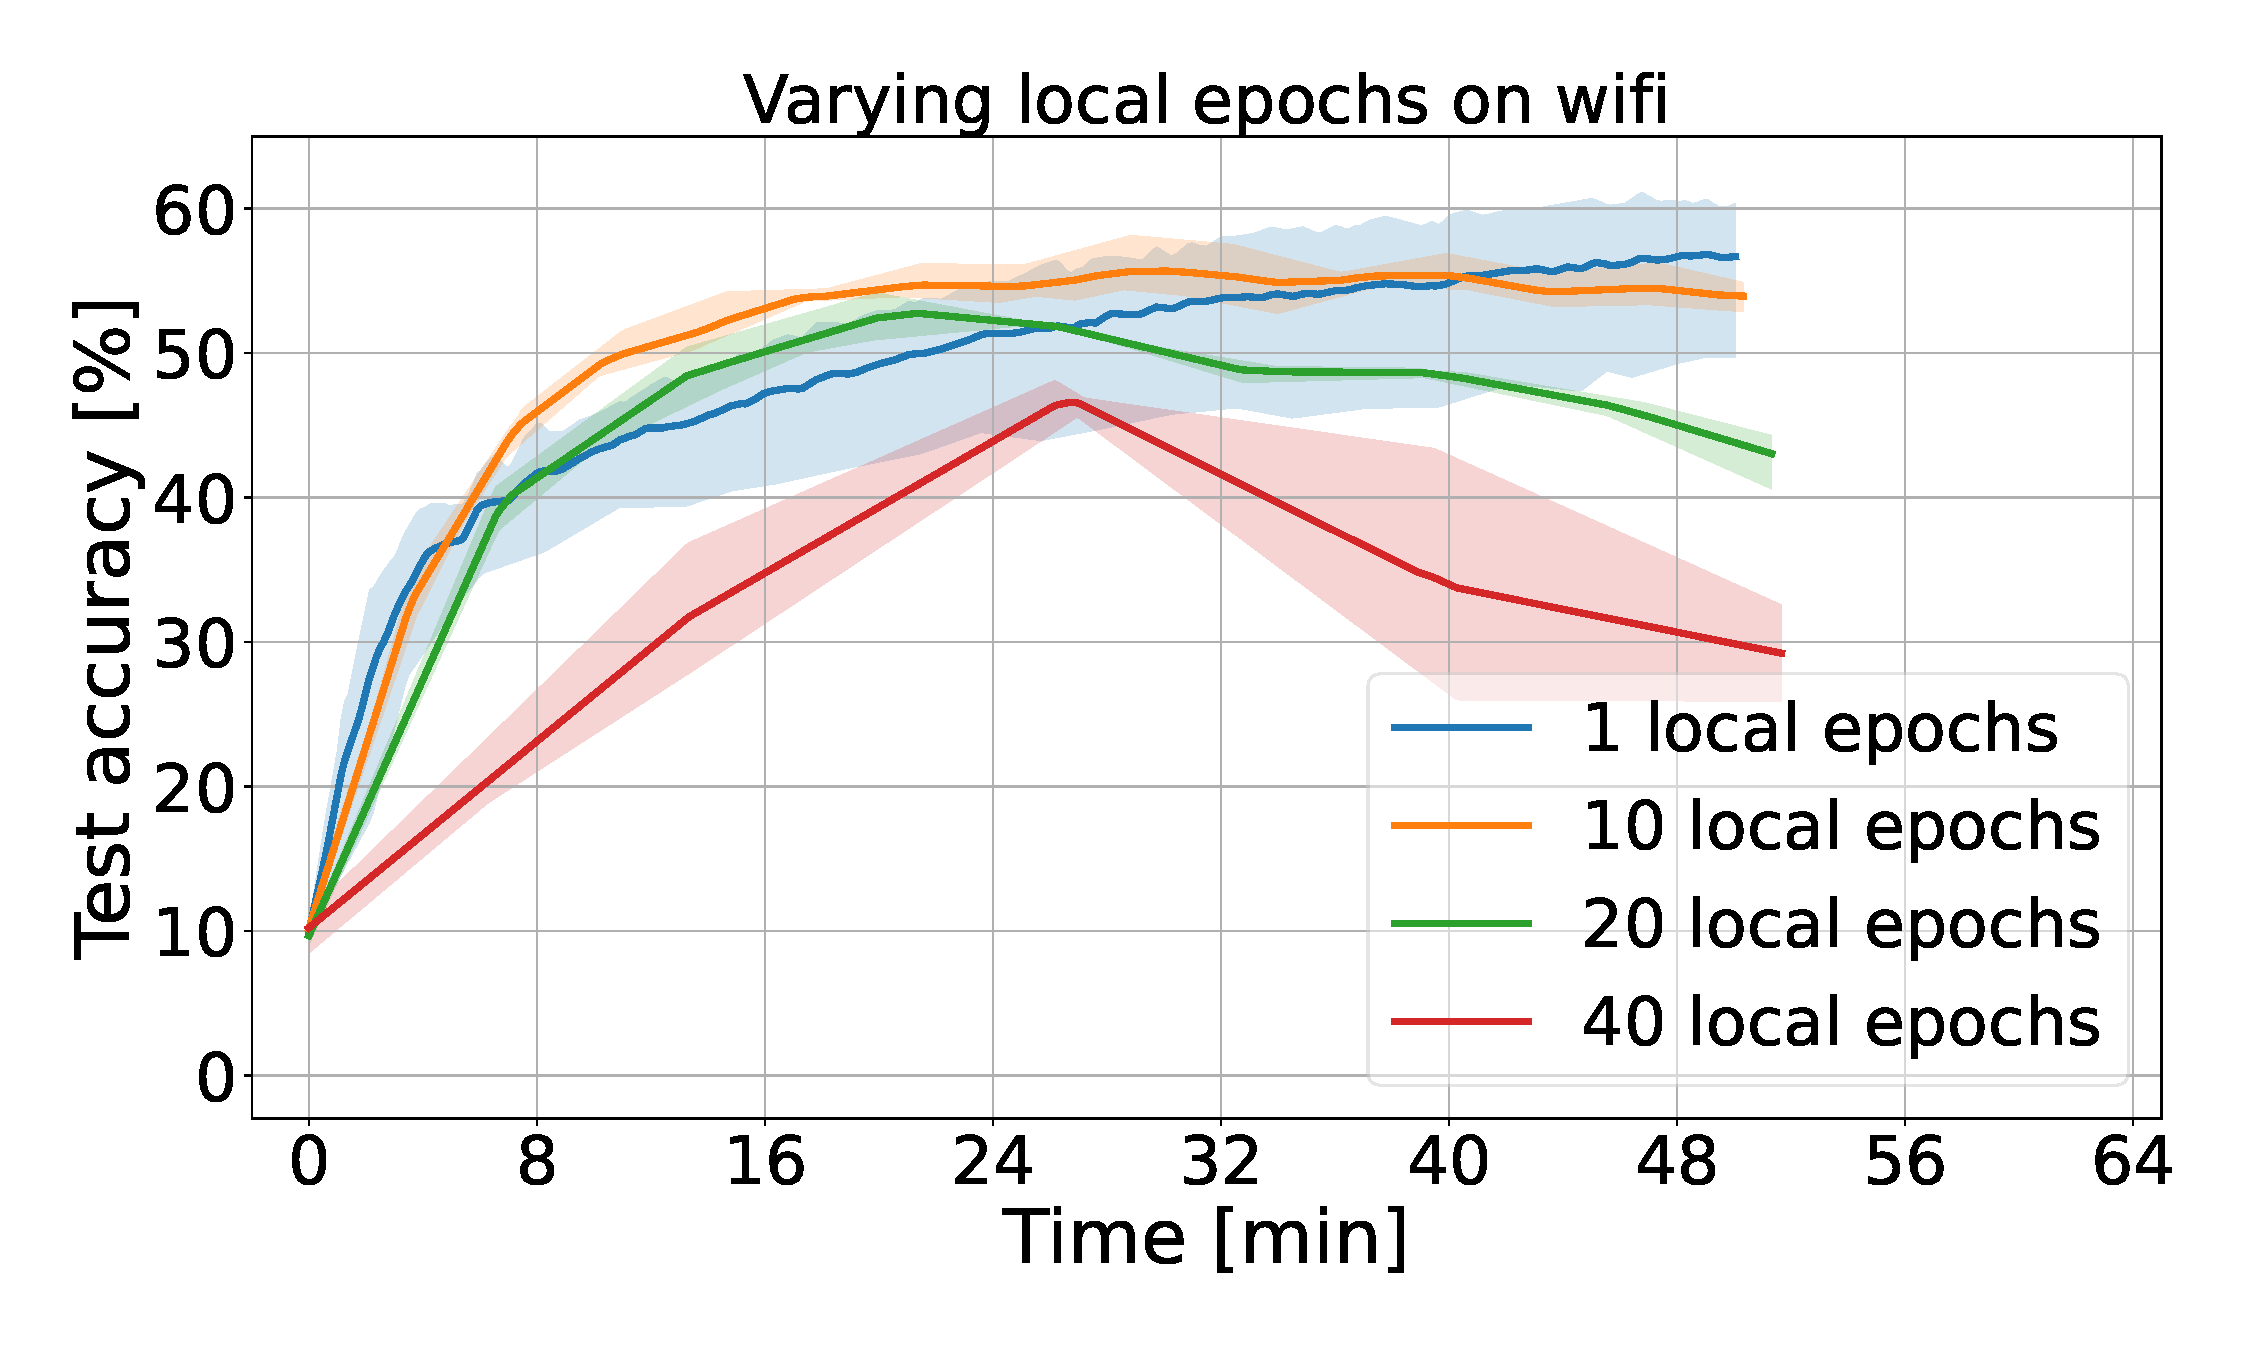
\includegraphics[width=\linewidth]{imgs/time_avg_local_epochs_wifi.pdf}
    \caption{Effect of the number of local epochs ($E$) using the Raspberry Pi setup on ethernet (top) and Wi-Fi (bottom).
    The lines show the mean accuracy of three repetitions, while the shaded areas outline the at any time best and worst of the repetitions.
    The legend also displays the number of rounds ($L$) each experiment completed before a timeout of 50 min.
}
    \label{fig:rpi-local-epochs}
\end{figure}\noindent
Table \ref{tab:main} shows the results of repeated experiments investigating different parameter choices after $L=20$ communication rounds.
% Redigér ikke tabel direkte, men redigér table_multirun.py
\begin{table}[htb!]
    \centering
    \begin{tabular}{llll}
       \hline
        \multicolumn{4}{c}{Local epochs ($E$)}\\
        1 & 10 & 20 & 40 \\
       \hline
$48.0 \pm 0.9$ & \textbf{ 52.2 $\pm$ 2.0 } & $37.6 \pm 2.4$ & $22.2 \pm 2.0$ \\
        \multicolumn{4}{c}{Clients samped ($S$)}\\
        5 & 10 & 20 & 40 \\
       \hline
        $35.4 \pm 4.8$ & $37.4 \pm 2.6$ & \textbf{ 38.1 $\pm$ 2.0 } & \textbf{ 38.1 $\pm$ 2.5 } \\
        \multicolumn{4}{c}{Class balance ($\alpha$)}\\
        0.01 & 1.0 & 100.0 & iid. \\
       \hline
        $10.3 \pm 0.6$ & $36.7 \pm 2.4$ & $42.6 \pm 3.4$ & \textbf{ 43.4 $\pm$ 2.5  }\\
        \multicolumn{4}{c}{FedDF: Class balance ($\alpha$)}\\
        0.01 & 1.0 & 100.0 & iid. \\
       \hline
        $9.9 \pm 0.2$ & $55.8 \pm 0.1$ & $56.5 \pm 0.9$ & \textbf{ 58.3 $\pm$ 1.0 } \\
        \multicolumn{4}{c}{Noisy clients ($N_K$)}\\
        0 & 10 & 20 & 30 \\
       \hline
        \textbf{ 37.1 $\pm$ 1.3 } & $14.0 \pm 2.1$ & $10.3 \pm 0.4$ & $10.6 \pm 0.8$ \\
        \multicolumn{4}{c}{FedDF: Noisy clients ($N_K$)}\\
        0 & 10 & 20 & 30 \\
       \hline
        \textbf{ 54.5 $\pm $ 0.4 } & $52.0 \pm 2.9$ & $51.6 \pm 1.9$ & $42.9 \pm 0.3$ \\
\end{tabular}
    \caption{
    Final test accuracies [\%] of FL models over $K=40$ clients when running for fixed $L=20$ communication rounds.
    Where nothing else is stated, parameters correspond to Table \ref{tab:baseline}.
    Each run is repeated five times to produce an approximate 95\%\ confidence interval.
    }
    \label{tab:main}
\end{table}

\section{DISCUSSION}%
\label{sec:discussion}

Firstly, the results show that model convergence is possible even though data is distributed across devices; a conclusion substantiated by the fact that continuing the $E=1$ training resulted in 95\pro\ of centralised learning performance which is shown in Appendix Table \ref{app:centralised}.

From the Raspberry Pi experiments on Figure \ref{fig:rpi-local-epochs}, we initially note that many accuracy curves fall during much of the learning.
This effect is continually worse with more local epochs.
We attribute this problematic behaviour to overfitting towards training sets, and, to check this explanation, visualise test performances during local epochs on Figure \ref{fig:accuracy}.
Here, training accuracy on each client skyrockets during local epochs while the training accuracy plummets.
% TODO: Hard to read
The direct mitigation is to perform a structured hyperparameter search where better regularising measures for this task are tested.
% TODO: Hard to read sentence
A more general idea is to perform local early stopping, but designing such a rule is non-trivial as we observe examples of the global, average model improving even though all local models overfit, as seen in early communication rounds and during the less biased learning for $E=10$ shown on Appendix Figure \ref{fig:accuracy2}.


When focusing on early learning less impacted by overfitting, the Raspberry Pi timing results reveal that it does not always hold that fewer local epochs are better.
More local epochs can be optimal if training time is limited, as seen in minutes 5 to 15 using Ethernet and minutes 5 to 40 for Wi-Fi.
During this time, the higher number of local epochs result in more time spent on training and less on communication, explaining why the this effect is most evident on relatively slow Wi-Fi.
There thus exists a trade-off where $E$ should not be too high to induce overfitting but not too low to slow down the rate of training data seen.
When choosing this parameter, practitioners should be mindful of available training time and communication latencies in the system.
\begin{figure}[htb!]
    \centering
        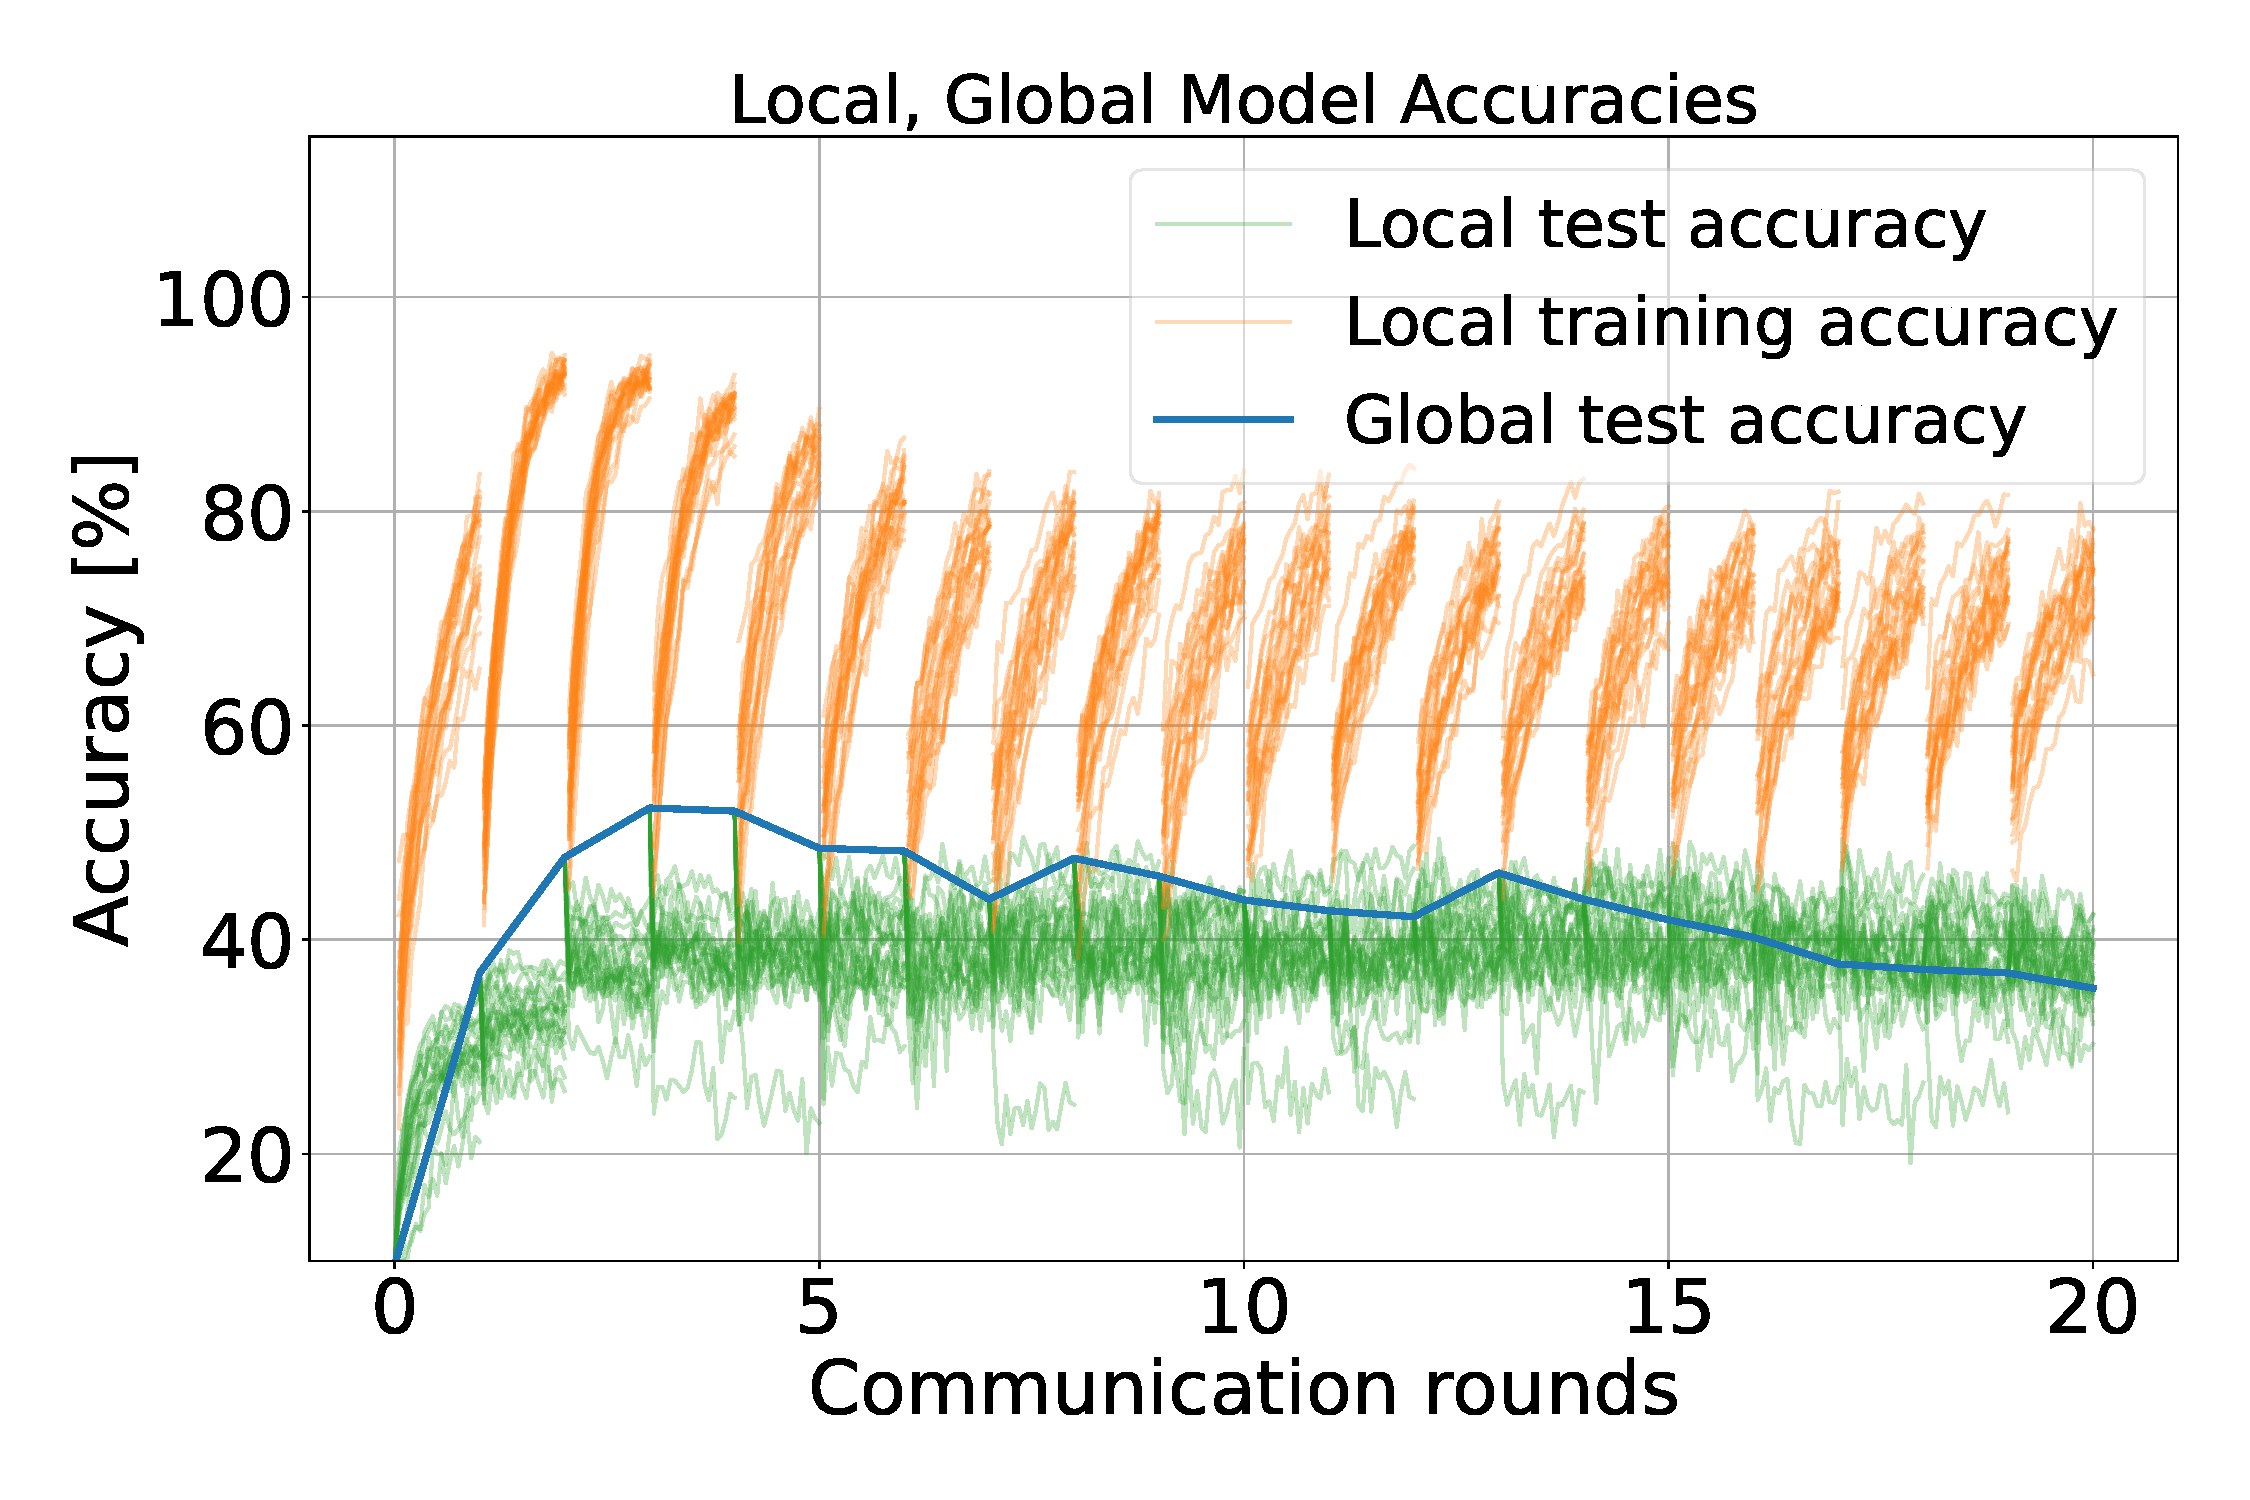
\includegraphics[width=\linewidth]{imgs/accuracy.pdf}
    \caption{
        A training trajectory when recording running accuracies on each client in each communication round where each faint line corresponds to $E=20$ local epochs performances of each of the $S=20$ sampled clients.
        For the $E=10$ case, see Appendix Figure \ref{fig:accuracy2}.
    }
    \label{fig:accuracy}
\end{figure}\noindent

\noindent
When running for a fixed number of rounds, as shown in Table \ref{tab:main}, computational and communicational effects are disregarded, and $E=10$ appears optimally as a compromise between under- and overfitting.
% TODO: Too wordy maybe
For the number of clients sampled each round $S$, we note that even though datasets are somewhat imbalanced, $\alpha=1$, FedAvg performs the same both when sampling half of the clients and when sampling all of the clients.
Even using only five clients each round, the accuracy ended at $93 \pro$ of all 40, emphasising the stability of model averaging.
This difference is largest in early rounds where lower values of $S$ induce slower convergence, also visualised in Appendix Figure \ref{fig:s}.

However, the class balance results show that this stability was removed when lowering $\alpha$ to $0.01$.
The learning improved significantly when training on more balanced classification tasks such as $\alpha=100$ or iid.

For the FedDF experiments with the same hyperparameters, a generally much higher level of performance is noted.
We speculate that the distillation procedure avoids the detrimental impact of the overfitted local models by performing a model fusion without averaging over big, bias-inducing parameters.
This is backed up by Figure \ref{fig:alpha} where the problem of long-term falling performance is removed when using FedDF.
Empirical prediction probability distributions might thus give a more robust characteristic of the learned knowledge than the model weights themselves.

\begin{figure}[H]
    \centering
         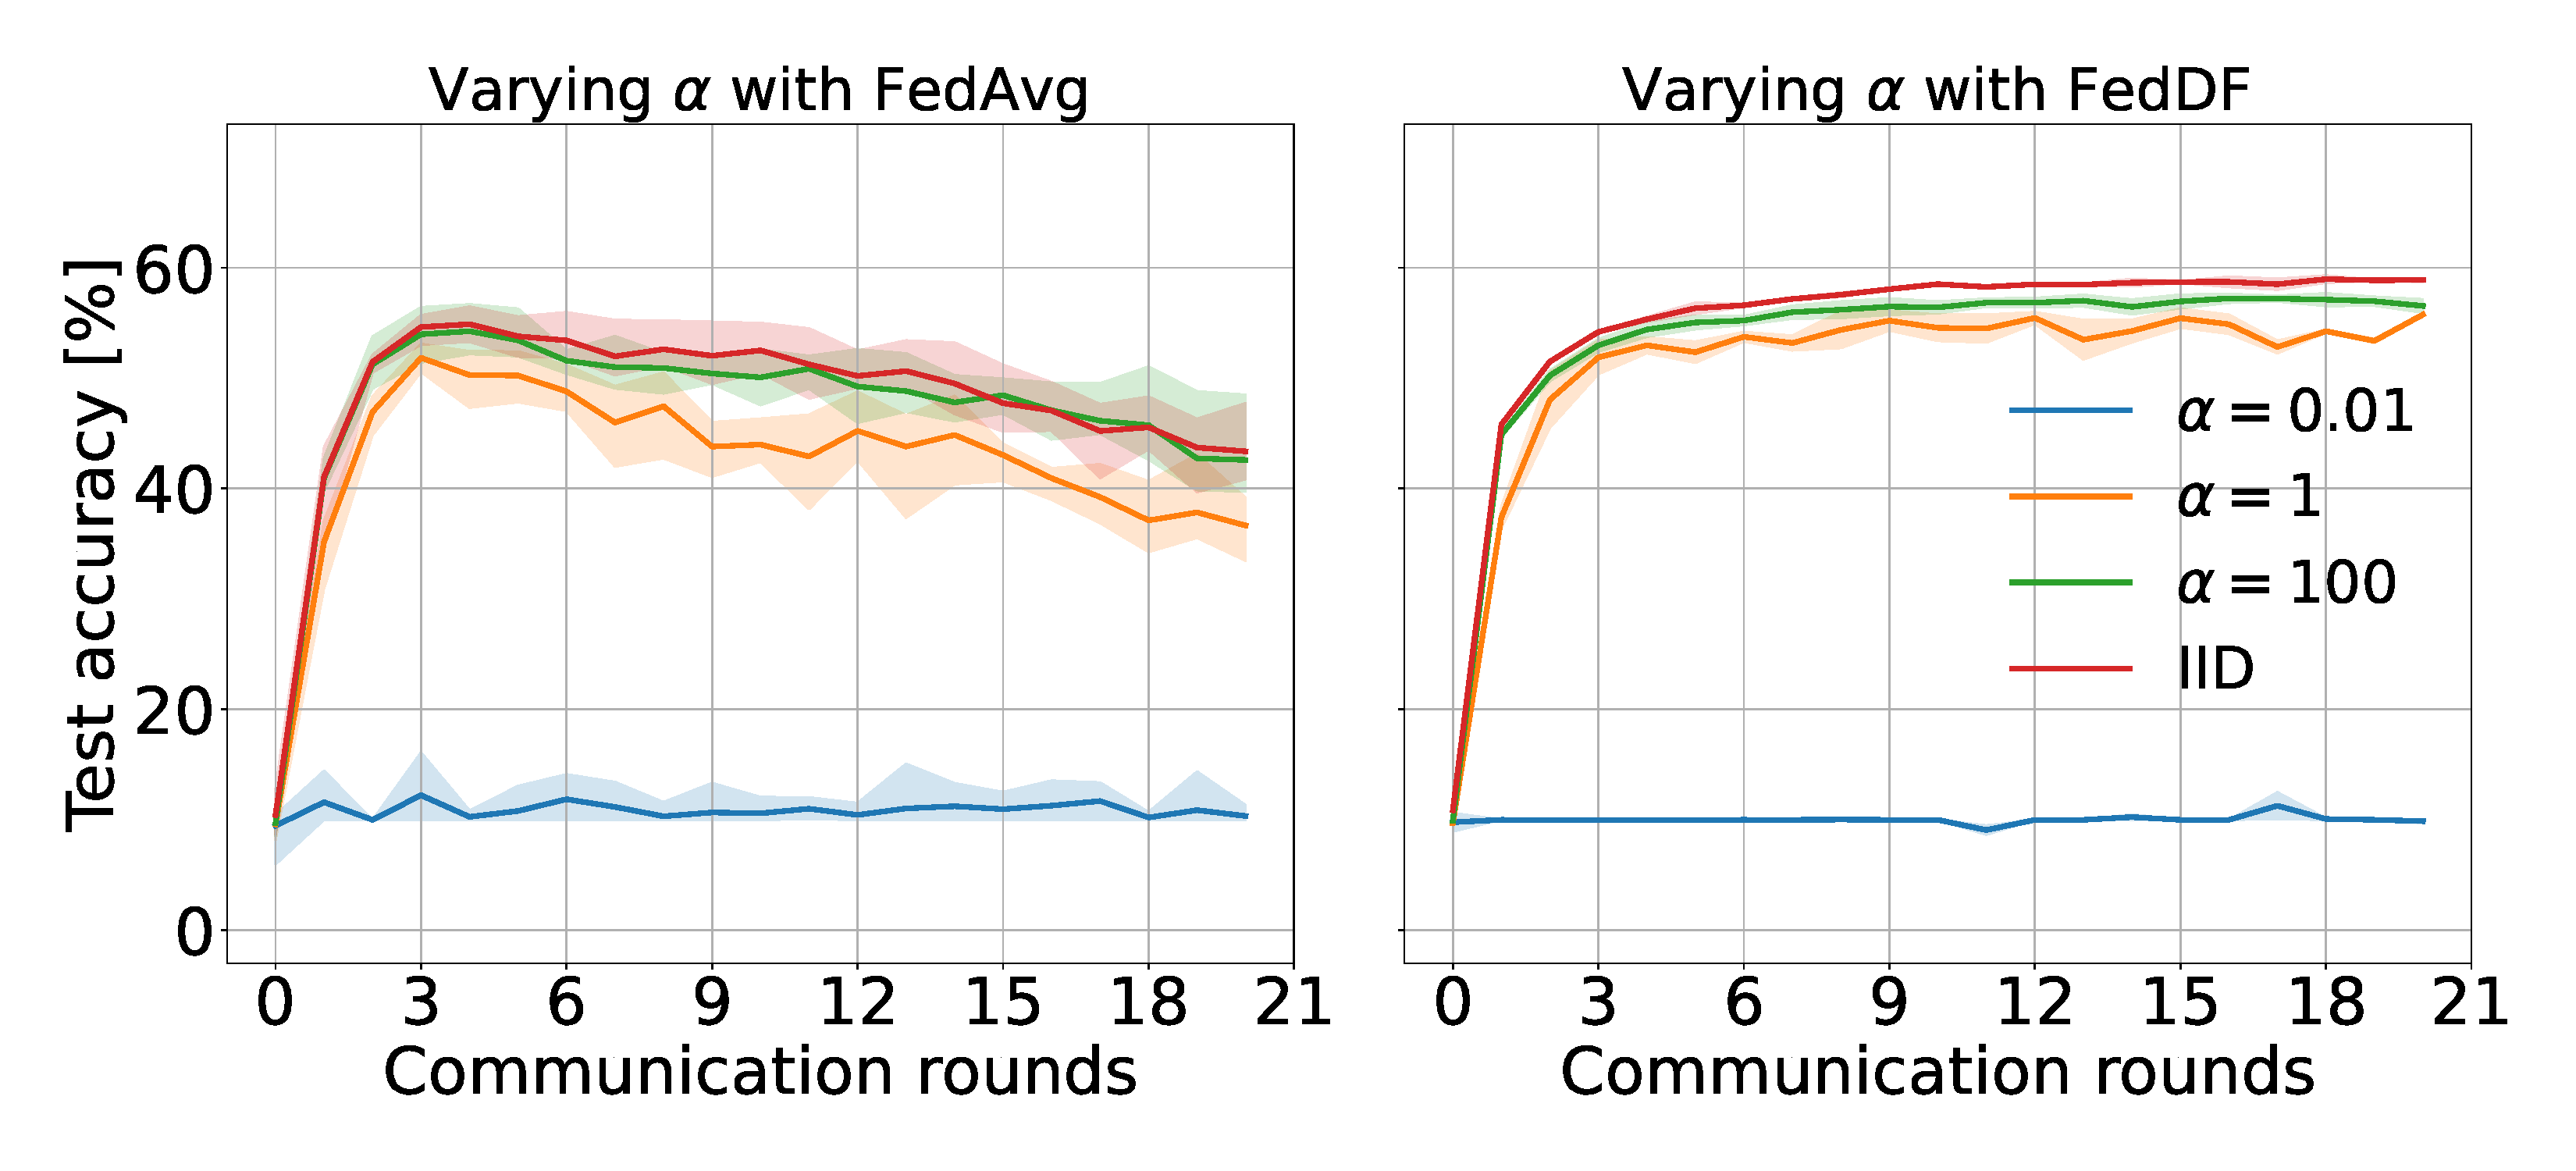
\includegraphics[width=\linewidth]{imgs/feddf-alpha.pdf}
    \caption{
    Performance of the global model on the test set over communication rounds when varying data imbalance using both FedAvg (left) and FedDF (right).
    The lines indicate the mean performance of multiple runs, with the coloured areas outlining the least and most performant repetition at any run.
    The FedAvg experiments were repeated five times, with the much slower FedDF experiments only being run twice.
    }
    \label{fig:alpha}
\end{figure}\noindent

\noindent
This added robustness is strongly exemplified for FedDF in the noise experiments.
Here, having 10 out of the 40 data partitions being noisy ruins the performance of FedAvg thoroughly, while FedDF can perform reasonably even at 30 out of 40.
Yet again, averaging probabilities instead of model weights appears to minimise the negative impact of fusing models with heterogeneous parameter values.

Though data label difference was simulated, use-cases such as smartphone computer vision or virtual keyboard language modeling have user data distributions that are much more diverse, e.g. one user only photographing their dog and another only landscapes, requiring analysis of data variety.
In addition to these learning considerations, practitioners should be aware of the fact that FL is not the entire solution to user privacy as user data might be recoverable from trained models weights.
To mitigate this, FL can be combined with differential privacy methods \cite{xiong2020ldp} to obtain maximally safe learning.

\subsection{Conclusions}
The case study performed in this project demonstrated that privacy-preserving learning on physical devices is possible as long as algorithmic choices are made with communication efficiency and robustness against data imbalance in mind.
Using the simple, foundational FedAvg algorithm, running more local training on devices raised overfitting, but fewer epochs raised communication overhead.
The distillation aggregation algorithm FedDF mitigated this overfitting and added robustness towards different data distributions at the cost of more computation on the central server.
To investigate multiple realistic learning tasks, including computer vision models with higher performance, a federatio of devices with more computing power than Raspberry Pi's, such as smartphones, could be subject to the same analysis.

\vfill
\pagebreak

\bibliographystyle{IEEEbib}
\bibliography{references}

\appendix
\section{Model}
\label{app:model}
The model architecture is described below, listing the sequential operations in the forward pass.
\begin{table}[htb!]
    \centering
    \begin{tabular}{l|p{5cm}}
            Layer type & Hyperparameters\\
            \hline
            2D Convolution & 1 in-channel, 16 out-channels, $3\times 3$ kernel, stride of 1\\
            ReLU activation\\
            2D Convolution & 16 in-channels, 32 out-channels, $3\times 3$ kernel, stride of 1\\
            ReLU activation\\
            2D MaxPooling & $2\times 2$ kernel, stride of 2, no padding, dilation of 1\\
            Dropout & $p=25\%$\\
            Flattening\\
            Linear w. bias & $6,272$ features in, 64 features out\\
            ReLU \\
            Dropout & $p=50\%$\\
            Linear w. bias & 64 features in, 10 features out
        \end{tabular}
\end{table}\noindent
\section{The Dirichlet Distribution For Data Imbalance}
\subsection{Impact of Dirichlet $\alpha$}%
Se Figure \ref{fig:splits} for illustration of varying degrees of data imbalance.
\label{app:dirplots}
\begin{figure}[htb!]
    \centering
        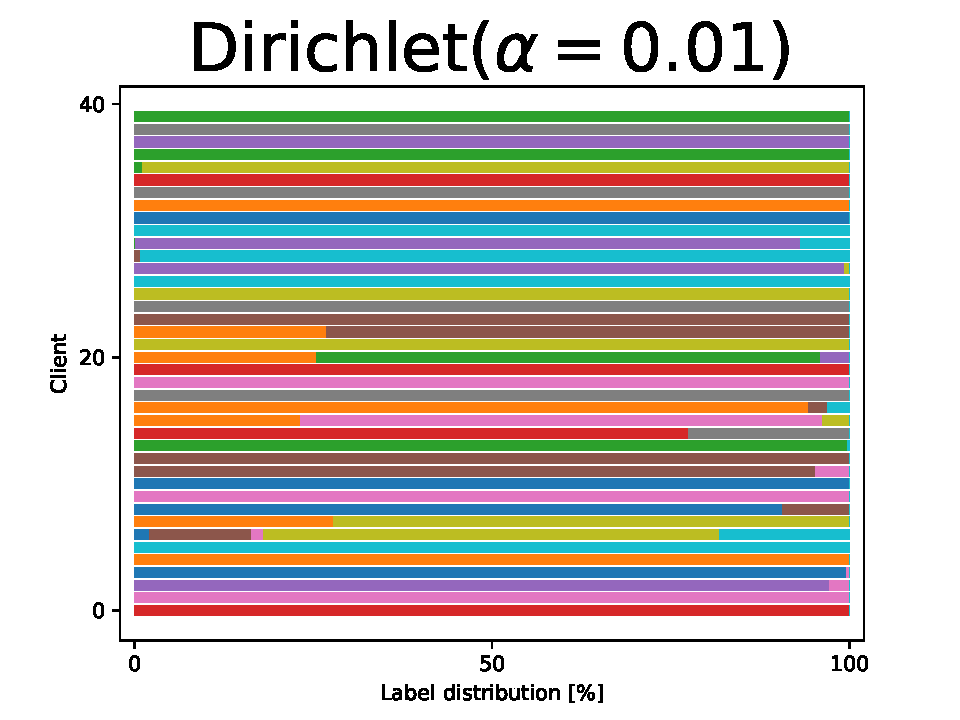
\includegraphics[width=0.49\linewidth]{imgs/splits(alpha=0.01)}
        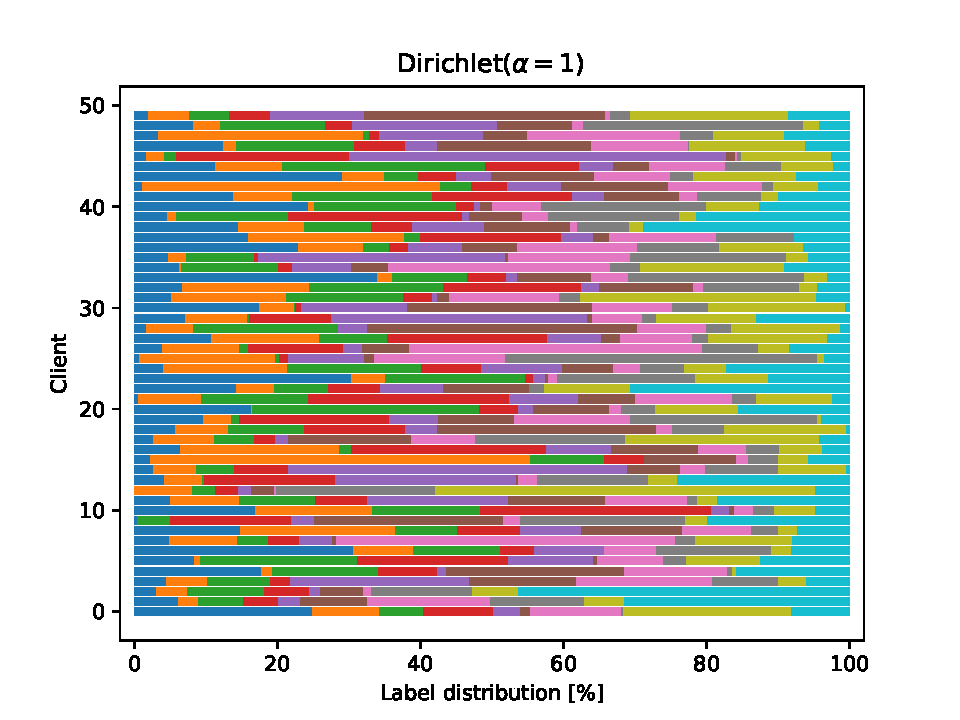
\includegraphics[width=0.49\linewidth]{imgs/splits(alpha=1).pdf}
        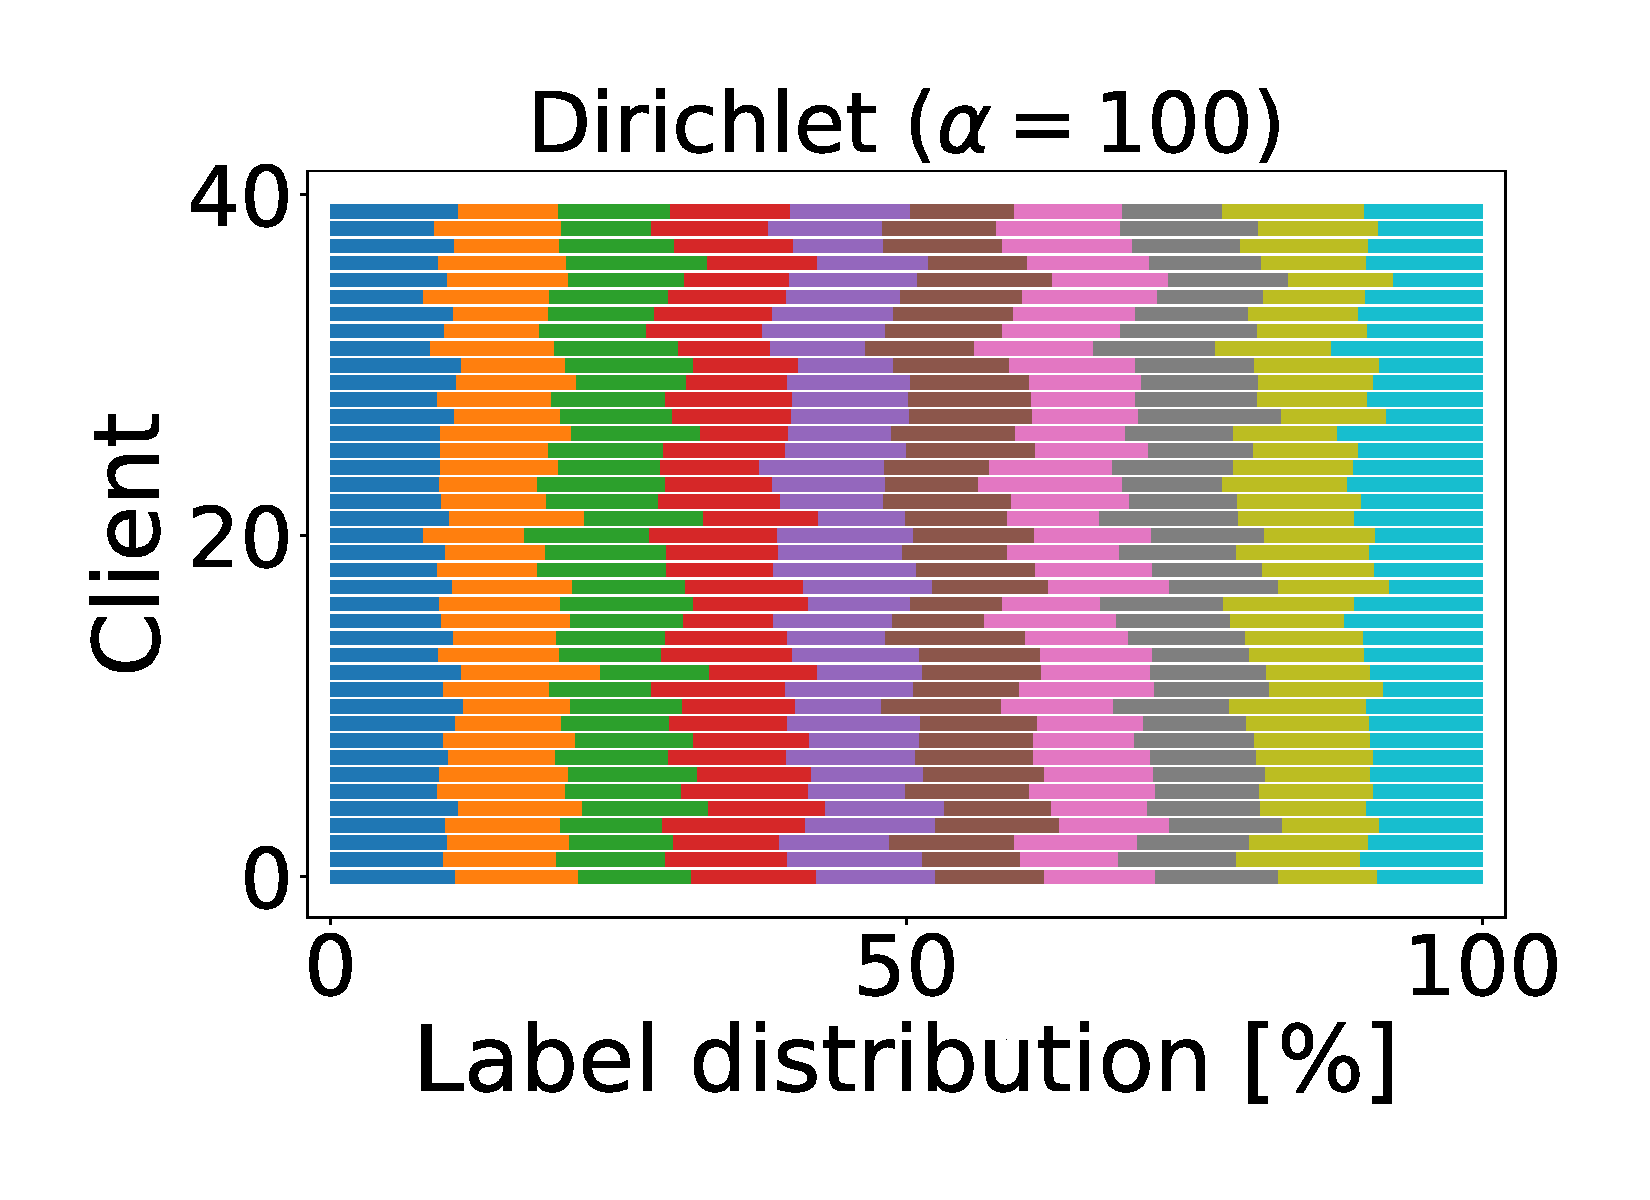
\includegraphics[width=0.49\linewidth]{imgs/splits(alpha=100)}
        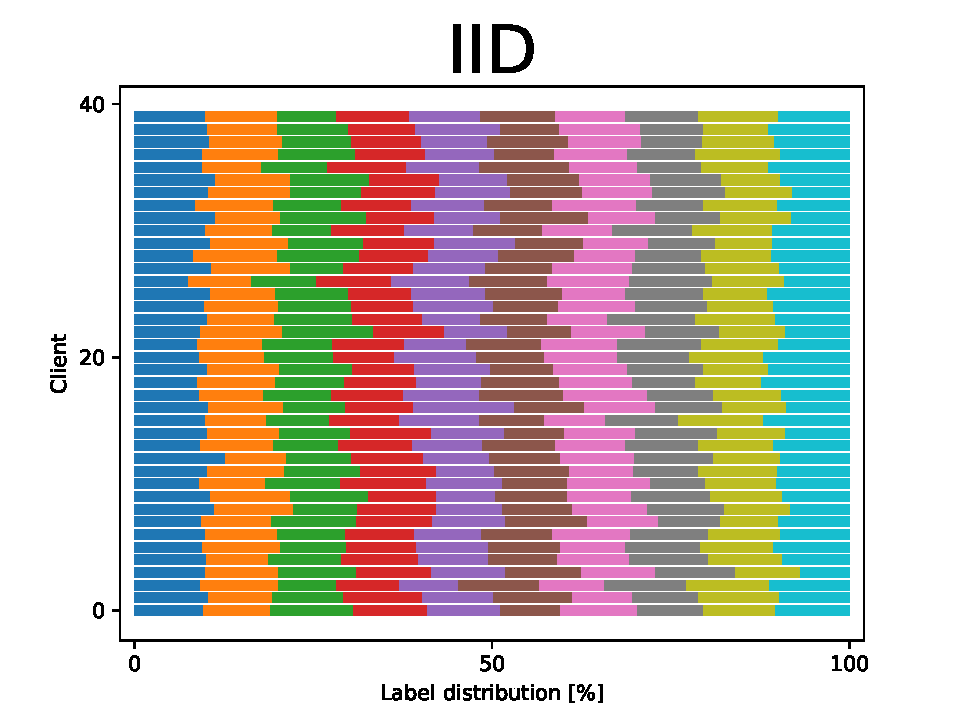
\includegraphics[width=0.49\linewidth]{imgs/splits(IID)}
    \caption{
        Example 10-class label distributions over 50 clients for each of the tested sampling paradigms, where each colour corresponds to a label and each row to a client.
    }
    \label{fig:splits}
\end{figure}\noindent


\subsection{Sampling Algorithm}%
\label{app:diralg}
Let $D$ denote a dataset of size $\len D$ with $l$ different labels, of which there are $\len D/l$ each.
The goal of the algorithm is to divide the dataset among $C$ clients, such that the label distribution, $\bm\pi_i$ of each client $i$, follows the same Dirichlet distribution, $\operatorname{Dir}(\bm\alpha)$, where every $\alpha_j\in\bm\alpha, j=1\ldots l$ is the same value.
For simplicity, the Dirichlet distribution will therefore be parametrized only by $\alpha$; $\operatorname{Dir}(\alpha)$.

The distributions are structured into a matrix $\mathbf P$ of size $ C\times l $, where the $i$'th row is $\bm\pi_i$.
The $ij$'th element, $P_{ij}$, is then the fraction of label $j$ on device $i$.
Furthermore, the sum of the $j$'th column is the relative usage of label $j$ scaled by the number of clients, $C$.
As such, for every label to be used equally much, every column should sum to $C/l$.
If any columns sum to more, the corresponding labels are oversampled, and so all of $\bm P$ needs to be normalized to make the largest column-sum equal $C/l$, causing some of the data to not be used.

A measure, $u$, is needed to determine how close $\mathbf P$ is to achieving the goal of making every column sum to the same.
The lowest value of this measure should be achieved for a $\mathbf P$ where every column sums to $C/l$, while it should be progressively higher for poorer $\mathbf P$'s.
We chose the L1 norm of difference in column sums and $C/l$:
\begin{equation*}
    u(\mathbf P) = \sum_{j=1}^{l} \len{\frac{C}{l} - \sum_{i=1}^{C} P_{ij}}
\end{equation*}
Similarly, standard deviation or the reciprocal of the entropy could be used.

The final thing to keep in mind before the algorithm is introduced is that reordering $\bm\pi_i$ makes it equally likely to be sampled from $ \operatorname{Dir}(\alpha) $.

The algorithm changes the ordering within each $\bm\pi_i$ iteratively, until $u(\mathbf P)$ is no longer lowered.
The full algorithm is shown with pseudocode in Algorithm \ref{alg:dir}.
\begin{algorithm}
\caption{Dirichlet sampling algorithm}
\label{alg:dir}
\begin{algorithmic}
\For{$i$ from 1 to $C$}\Comment{Initialize $\mathbf P$}
    \State $\mathbf P_i \gets \operatorname{Dir}(\alpha)$
\EndFor
\Loop
    \State{$d \gets $ Map()}\Comment{Map swaps to $u$ values}
    \For{$i$ from 1 to $C$}\Comment{Do all possible swaps}
        \ForAll{$(j_1, j_2)\in (1\ldots l)\times (1\ldots l), j_1\neq j_2$}
            \State{Swap $P_{ij_1}$ and $ P_{ij_2} $}
            \State{$ d[ (i, j_1, j_2) ] \gets u(\mathbf P)$ }
            \State{Swap $P_{ij_1}$ and $ P_{ij_2} $ back}
        \EndFor
    \EndFor
    \If{$\min(d) < u(\mathbf P)$}
        \State $ i, j_1, j_2 \gets \operatorname{argmin}(d) $
        \State{Swap $P_{ij_1}$ and $ P_{ij_2} $}
    \Else
        \State{Break}\Comment{No improvement possible}
    \EndIf
\EndLoop
\State{$ \bm\pi \gets \sum_{i=1}^{C} \bm\pi_i $}
\State{$ \mathbf P \gets \mathbf P / \max(\bm\pi) $}
\Comment{Normalize $\mathbf P$ by most sampled label}
\end{algorithmic}
\end{algorithm}
The final $\mathbf P$ produced by the algorithm is normalized such that all data points with the most sampled labels are used exactly once.

In general, labels were found to be sampled more evenly for higher values of $C$ and $\alpha$.
Running the algorithm for $C=100$ and $\alpha=0.01$ 100 times showed an average undersampling of less than 1\pro\ with the largest undersampling being 3.3\pro.
Only rarely was any one label undersampled by more than 5\pro, a sign of the strength of the algorithm, even for a low value of $\alpha$.

\section{Further Results}%

\begin{figure}[htb!]
    \centering
        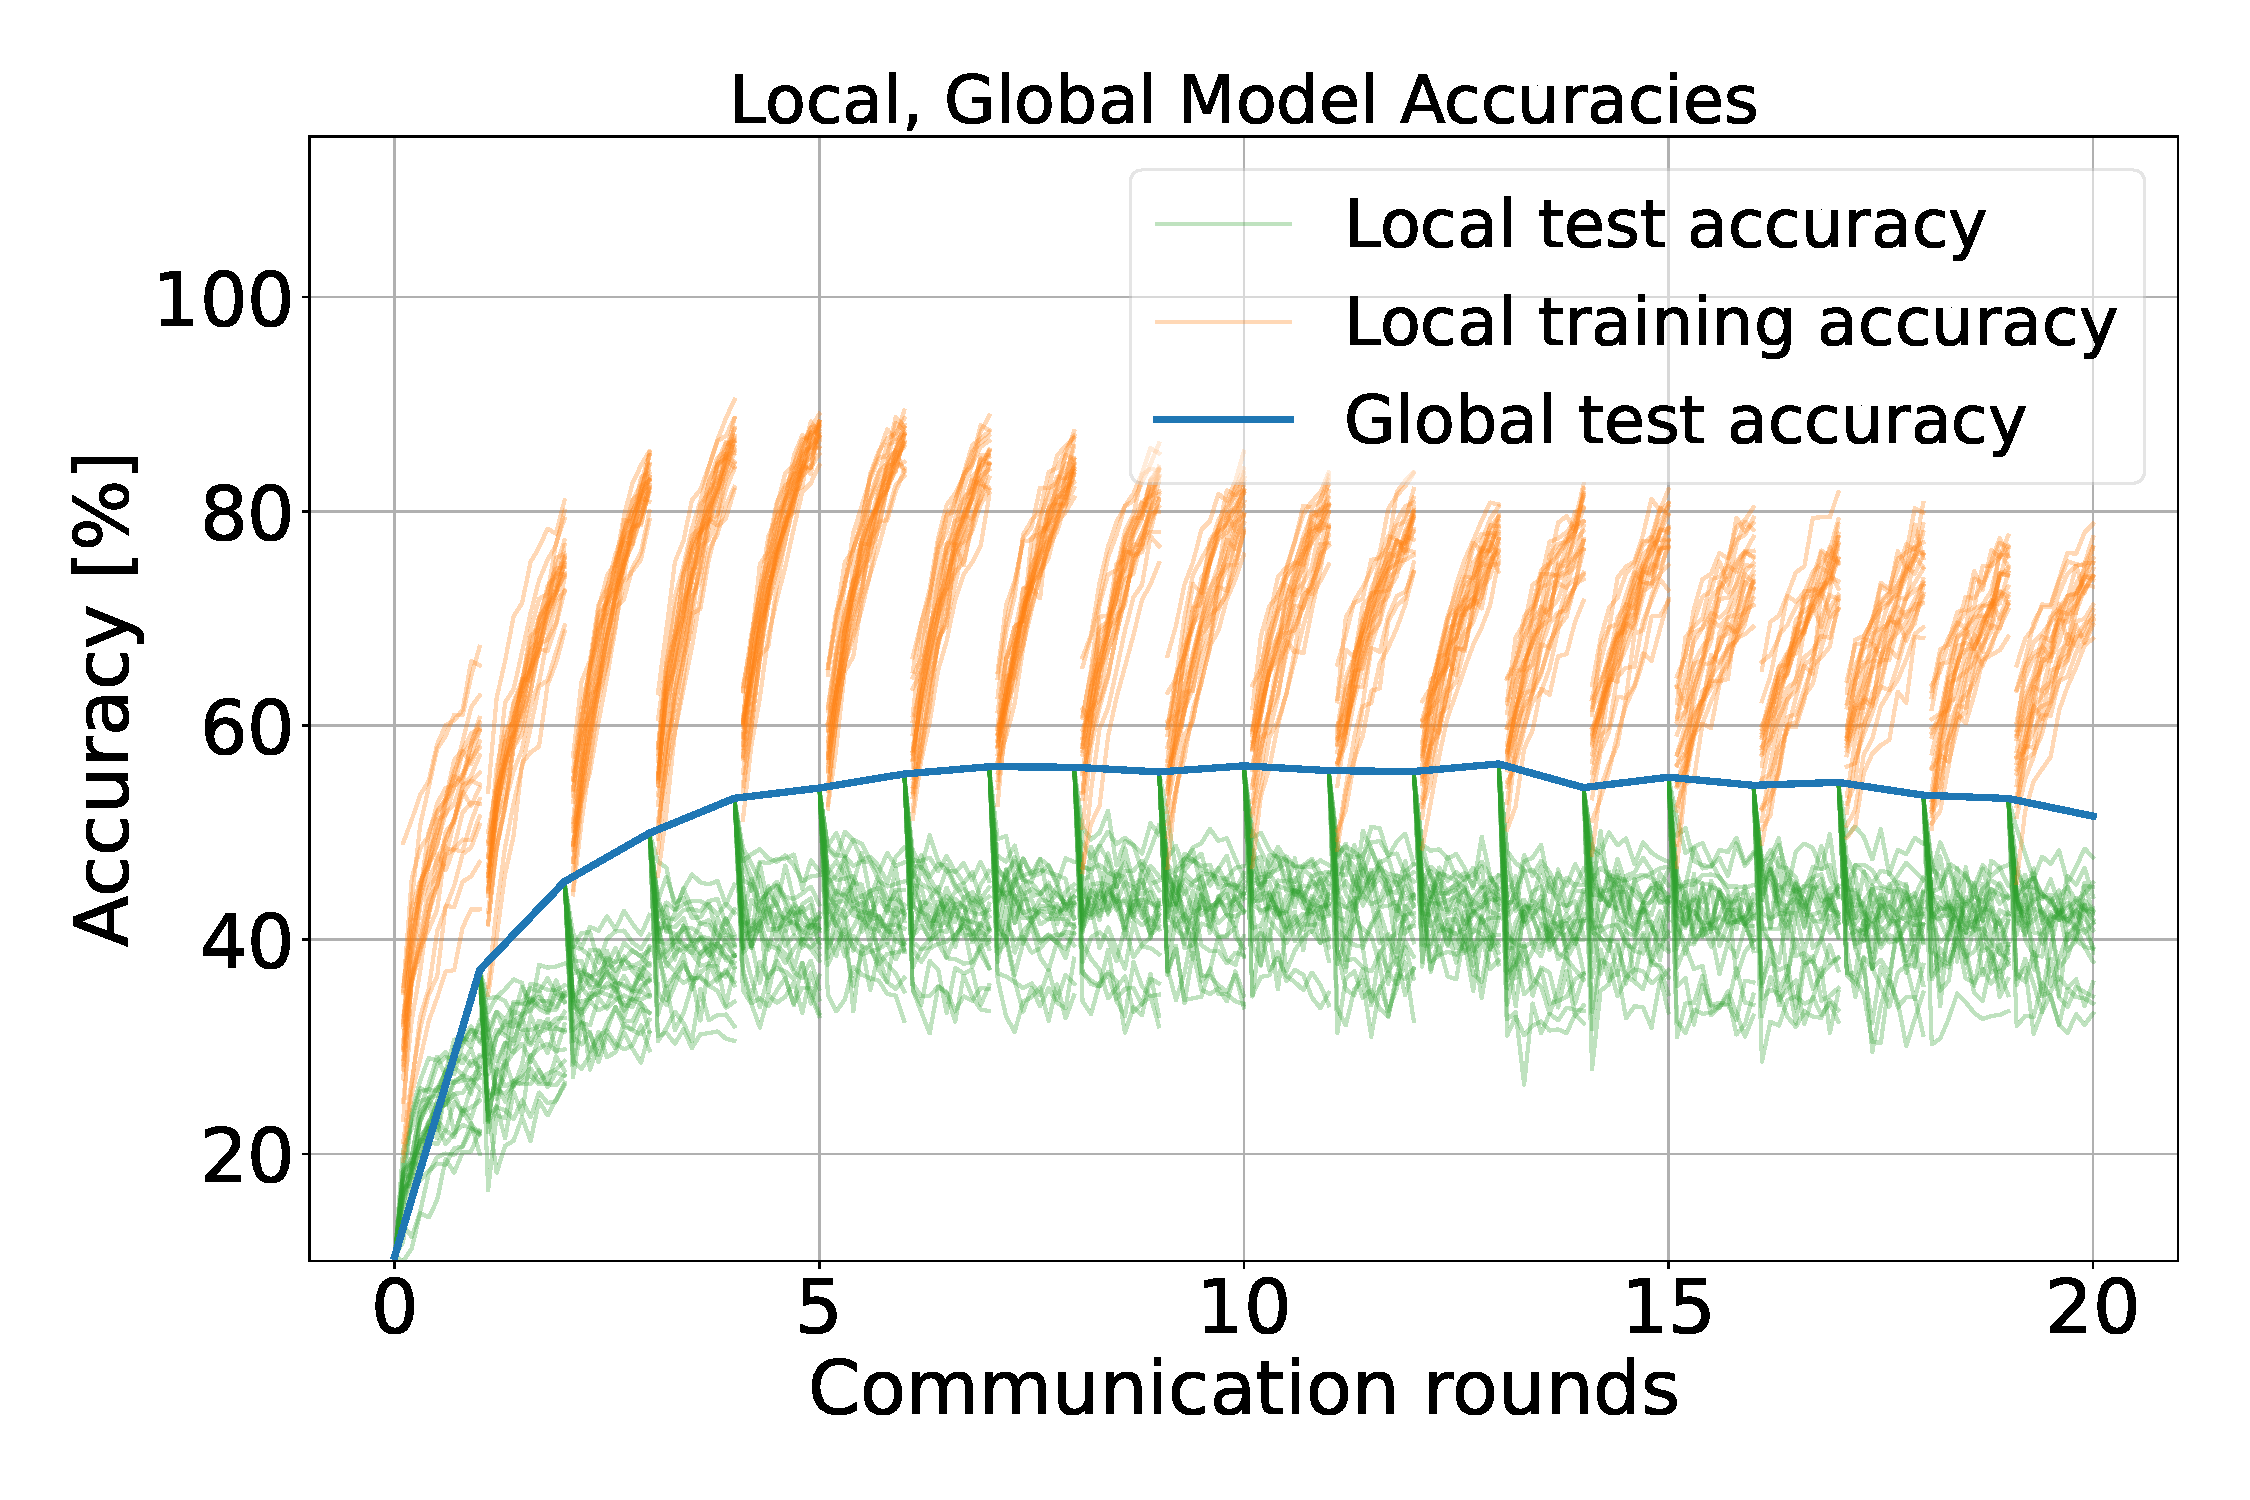
\includegraphics[width=\linewidth]{imgs/accuracyE10.pdf}
    \caption{
        A version of \ref{fig:accuracy} with $E=10$.
    }
    \label{fig:accuracy2}
\end{figure}\noindent

\begin{table}[htb!]
    \centering
        \begin{tabular}{lll}
            Algorithm & Steps before convergence & Final accuracy\\
            \hline
            FedAvg & 200 comm. rounds & 62.1 \%\\
            Centralised & 10 full epochs & 65.3 \%
        \end{tabular}
    \caption{
        Test set accuracy when running the above learning algorithms until test set accuracy stopped improving for 3 steps.
        The used FedAvg algorithm used $E=1$ and otherwise baseline parameters presented in \ref{tab:baseline}.
        The centralised learning algorithm used the full training each epoch, but otherwise same optimization approach as FL.
    }
    \label{app:centralised}
\end{table}\noindent
\begin{figure}[htb!]
    \centering
    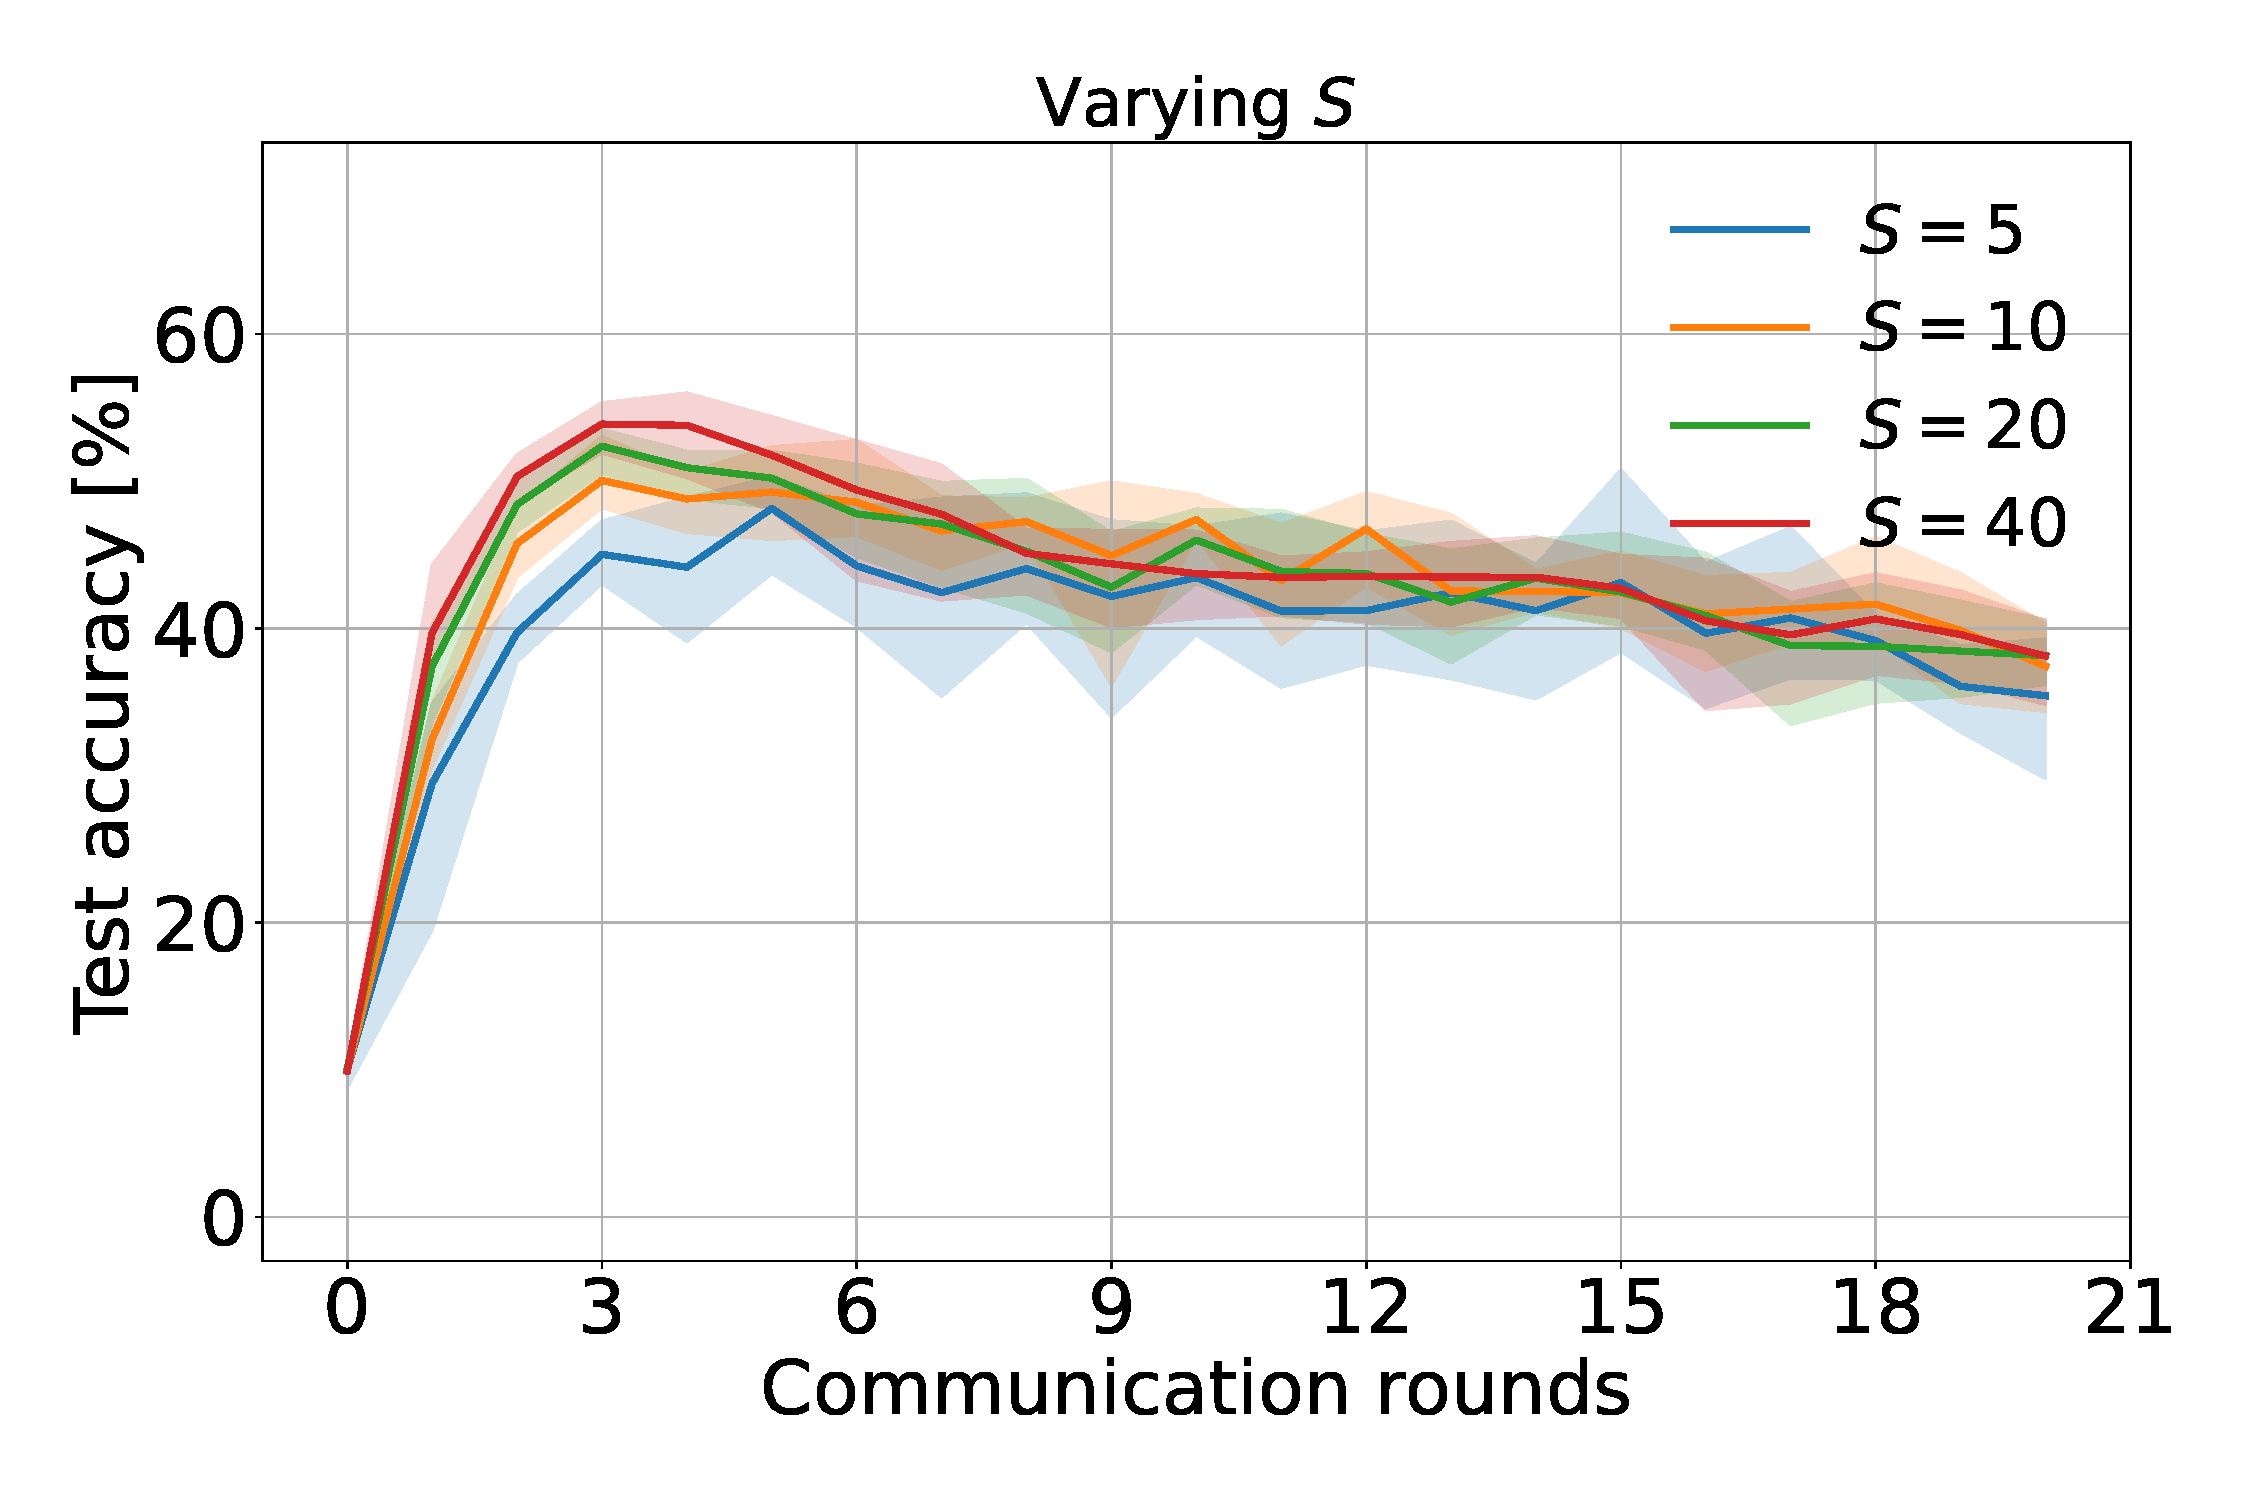
\includegraphics[width=\linewidth]{imgs/S.pdf}
    \caption{Performance of the global model on the test at different communication rounds with varying number of clients sampled per round, $S$.
    The lines indicate the mean performance of five runs, with the coloured areas outlining the least and most performant repetition at any run.}
    \label{fig:s}
\end{figure}\noindent


\end{document}
